\subsection{Pengenalan Quartus Prime}

Quartus Prime merupakan perangkat lunak CAD (computer-assisted design)
yang digunakan untuk desain rangkaian digital. Quartus Prime dikembangkan
oleh Altera. Versi Lite dari Quartus Prime dapat diunduh secara gratis
pada laman Altera\footnote{\url{http://dl.altera.com/?edition=lite}}.
Quartus Prime dapat dijalankan pada
platform Windows dan Linux.
Jendela utama dari Quartus Prime Lite dapat dilihat pada Gambar
\ref{fig:main_window}.

\begin{figure}
\centering
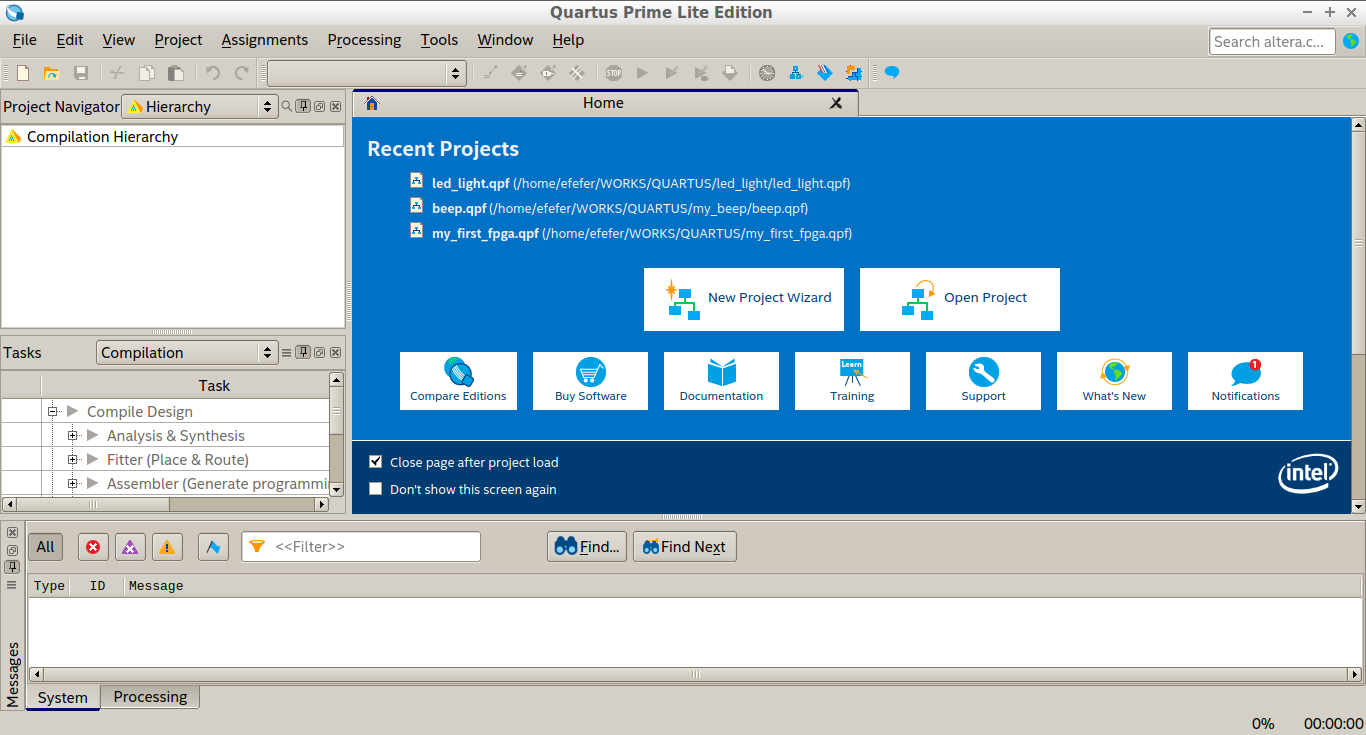
\includegraphics[width=\textwidth]{images/FirstOpen.png}
\par
\caption{Tampilan jendela utama Quartus Prime Lite}\label{fig:main_window}
\end{figure}

Dengan menggunakan CAD, setidaknya ada dua cara untuk
mendesain rangkaian digital:
\begin{itemize}
\item \textit{schematic capture}, dengan membuat skematik dari rangkaian yang
diinginkan.
\item menggunakan Hardware Description Language (HDL).
Dua jenis HDL yang paling populer adalah Verilog dan VHDL.
Kedua bahasa tersebut telah diadopsi sebagai IEEE Standard.
Pada tulisan ini akan digunakan Verilog.
\end{itemize}

Kita akan mulai dengan membuat project baru dan menambahkan skematik.

\subsection{Membuat project baru}
Berikut ini adalah langkah-langkah yang digunakan untuk membuat New Project
pada Quartus Prime Lite.

\framebox[1.1\width]{\textbf{Langkah 1}}
Pilih menu: \textbf{File $\rightarrow$ New Project Wizard}.
Jendela baru seperti pada gambar berikut akan
muncul.
Centang \textbf{Don't show me this introduction again} jika perlu.
Klik \textbf{Next}.
\begin{figure}[H]
\centering
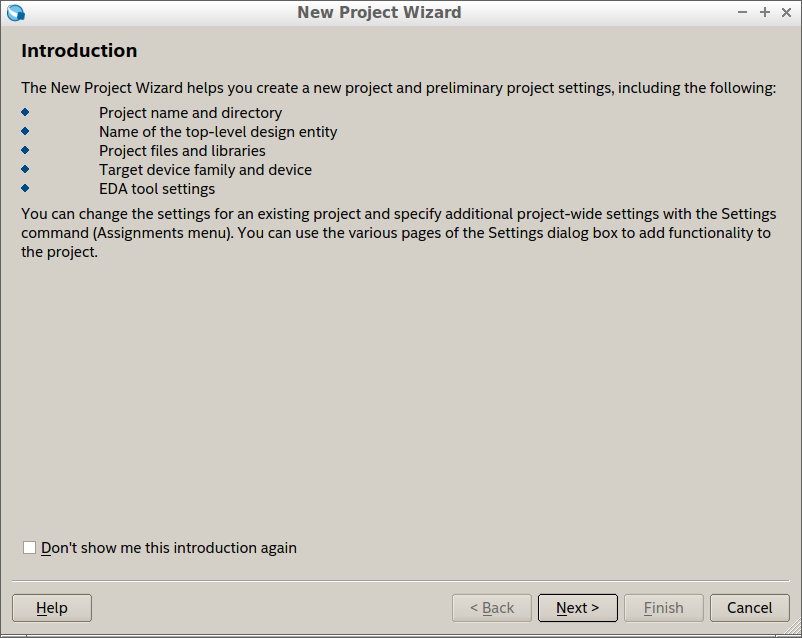
\includegraphics[width=0.5\textwidth]{images/NewProjectWizard_1.png}
\par
\end{figure}


\framebox[1.1\width]{\textbf{Langkah 2}}
Tentukan nama Project yang akan dibuat dan direktori di
mana file-file yang terkait dengan Project ini akan disimpan. Contoh
dapat dilihat pada gambar berikut. Setelah itu, klik \textbf{Next}
setelah semua isian diberikan.

\begin{figure}[H]
\centering
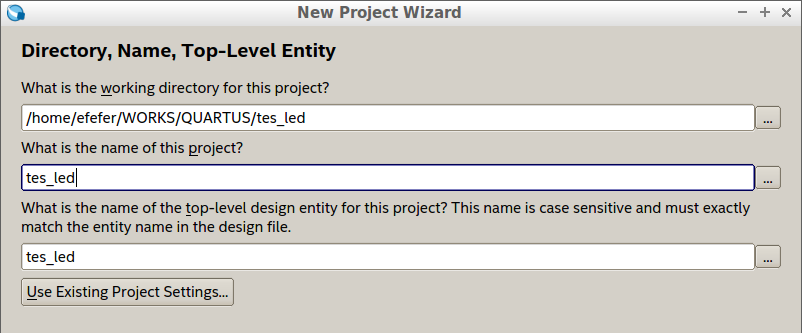
\includegraphics[width=0.5\textwidth]{images/NewProjectWizard_2.png}
\par
\end{figure}


\framebox[1.1\width]{\textbf{Langkah 3}}
Kita diminta untuk memilih jenis Project. Pilih \textbf{Empty Project}.
Setelah itu, klik \textbf{Next}.

\begin{figure}[H]
\centering
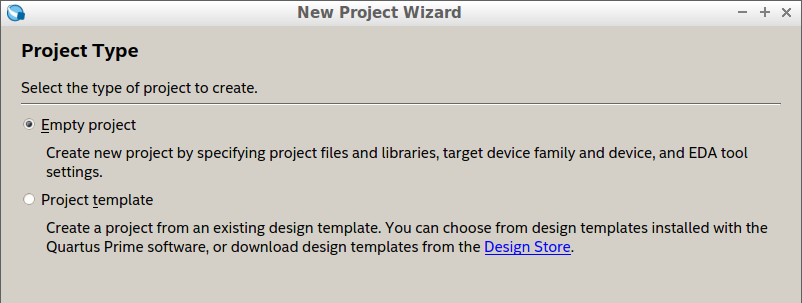
\includegraphics[width=0.5\textwidth]{images/NewProjectWizard_3.png}
\par
\end{figure}


\framebox[1.1\width]{\textbf{Langkah 4}}
Pada langkah ini kita dapat menambahkan file yang sudah ada ke Project
yang akan dibuat. Jika tidak ada langkah ini dapat dilewati.
Klik \textbf{Next}.

\begin{figure}[H]
\centering
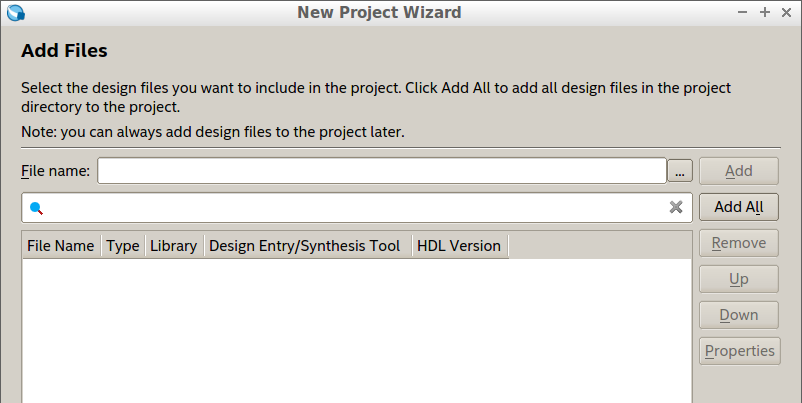
\includegraphics[width=0.5\textwidth]{images/NewProjectWizard_4.png}
\par
\end{figure}

\framebox[1.1\width]{\textbf{Langkah 5}}
Pada langkah ini, kita harus memilih \textbf{Device Family} dan
\textbf{Name}. Untuk \textbf{Device Family} pilih \textbf{Cyclone IV E}.

\begin{figure}[H]
\centering
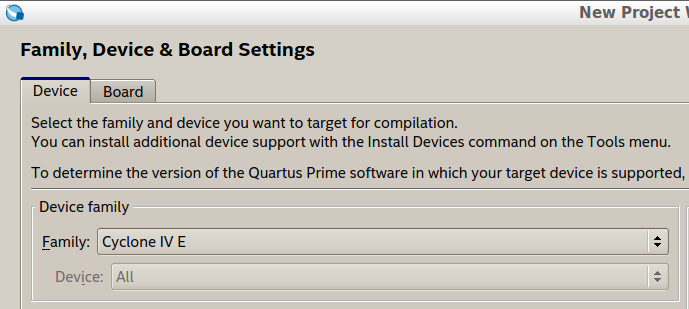
\includegraphics[width=0.5\textwidth]{images/NewProjectWizard_5_device_family.png}
\par
\end{figure}

Pada \textbf{Available Device} pilih \textbf{EP4CE6E22C8}.
Setelah itu, klik \textbf{Next}.

\begin{figure}[H]
\centering
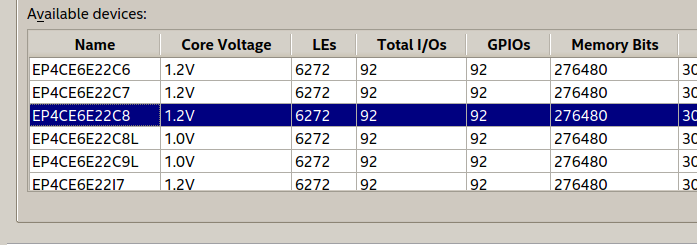
\includegraphics[width=0.5\textwidth]{images/NewProjectWizard_5_device_name.png}
\par
\end{figure}


\framebox[1.1\width]{\textbf{Langkah 6}}
Quartus akan meminta kita untuk memilih setting beberapa tools yang
mungkin digunakan. Untuk sementara pilih \textbf{None} untuk semua tools.
Setelah itu, klik \textbf{Next}.

\begin{figure}[H]
\centering
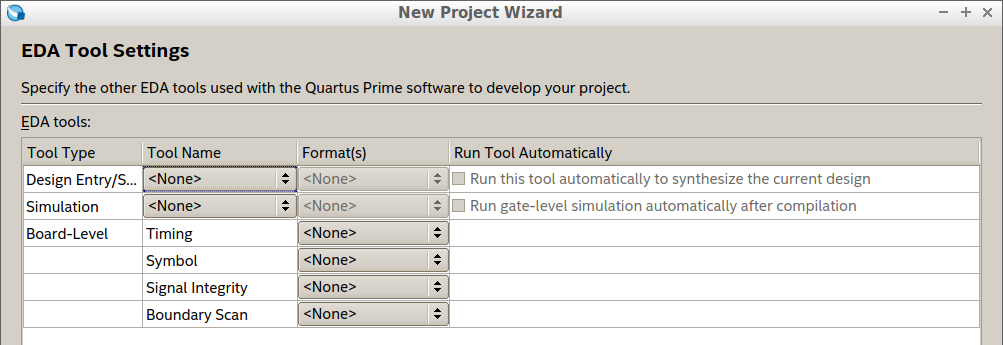
\includegraphics[width=0.5\textwidth]{images/NewProjectWizard_6.png}
\par
\end{figure}

\framebox[1.1\width]{\textbf{Langkah 7}}
Pada bagian akhir, Quartus akan memberikan Summary dari Project yang akan
dibuat. Setelah itu, klik \textbf{Finish}.
\begin{figure}[H]
\centering
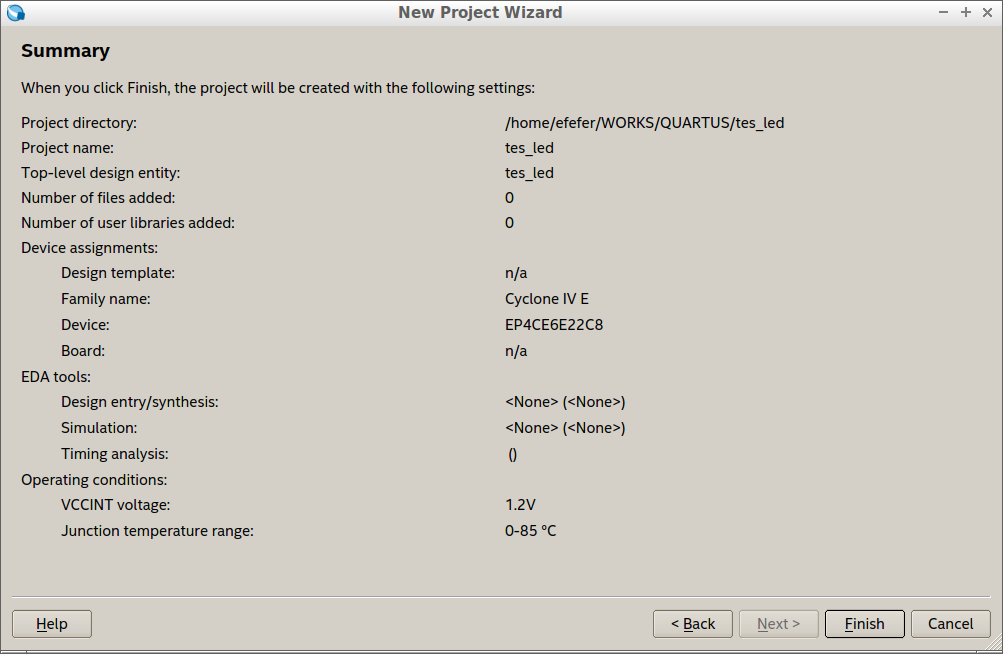
\includegraphics[width=0.5\textwidth]{images/NewProjectWizard_7.png}
\par
\end{figure}




\subsection{Menambahkan skematik baru}\label{subsec:skematik}

Skematik baru dapat ditambahkan ke dalam project dengan memilih menu
\textbf{File $\rightarrow$ New}. Pilih \textbf{New Diagram/Schematic File}, kemudian
\textbf{OK}.

\begin{figure}[H]
\centering
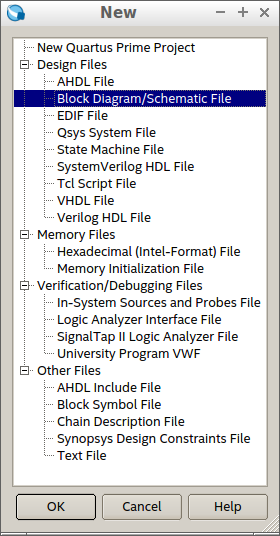
\includegraphics[scale=0.5]{images/NewSchematic.png}
\par
\end{figure}

File skematik kosong akan terbuka pada tab baru dengan nama \textbf{Block1.bdf}.
Kita dapat membuat skematik yang kita inginkan pada file ini.

\begin{figure}[H]
\centering
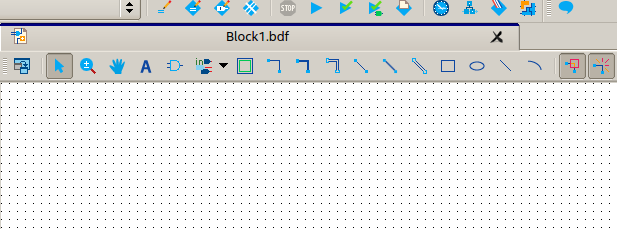
\includegraphics[scale=0.5]{images/EmptySchematic.png}
\par
\end{figure}

Untuk menambahkan komponen, dapat dilakukan dengan cara mengklik toolbar
\textbf{Symbol Tool}.

\begin{figure}[H]
\centering
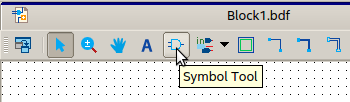
\includegraphics[scale=0.5]{images/SymbolTool.png}
\par
\end{figure}

Komponen yang ingin ditambahkan pada skematik dapat diperoleh dengan
ekspasi node \textbf{Libraries}, mencari komponen tersebut, dan memilihnya.
Misalkan kita ingin menambahkan gerbang AND dengan dua input, maka dapat dipilih
pada \textbf{primitives $\rightarrow$ logic $\rightarrow$ and2}. Klik
\textbf{OK} setelah komponen yang diinginkan telah dipilih.

\begin{figure}[H]
\centering
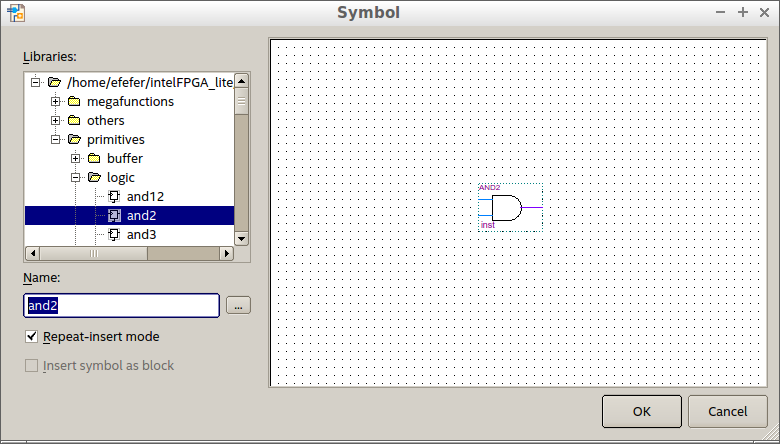
\includegraphics[scale=0.5]{images/BlockAnd.png}
\par
\end{figure}

Pemilihan komponen juga dapat dilakukan dengan mengetikkan nama komponen yang
diinginkan pada isian \textbf{Name}, misalnya \textbf{jkff} untuk J-K flip-flop.

Khusus untuk menambahkan komponen input dan output, dapat juga digunakan
toolbar \textbf{Pin Tool}.
\begin{figure}[H]
\centering
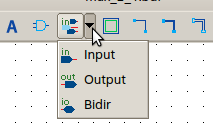
\includegraphics[scale=0.5]{images/PinTool.png}
\par
\end{figure}

Untuk menghubungkan antara satu komponen dengan komponen yang lain, dapat
digunakan \textbf{Orthogonal Node Tool}.
\begin{figure}[H]
\centering
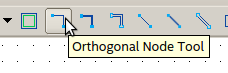
\includegraphics[scale=0.5]{images/OrthogonalNodeTool.png}
\par
\end{figure}

Berikut ini adalah contoh skematik untuk multiplexer 2-to-1:
\begin{figure}[H]
\centering
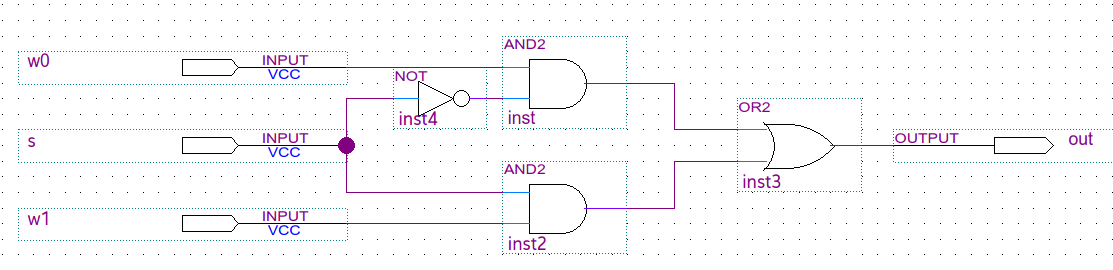
\includegraphics[width=\textwidth]{images/sch_mux_2_1.png}
\par
\end{figure}

Skematik ini kemudian dapat digunakan untuk proses lebih lanjut seperti
simulasi dan download ke hardware FPGA.

Menkonversi ke skematik ke simbol/blok sehingga dapat digunakan sebagai
bagian dari skematik lainnya: gunakan menu \textbf{File $\rightarrow$
Create/Update $\rightarrow$ Create Symbol Files for Current File}.

\begin{figure}[H]
{\centering
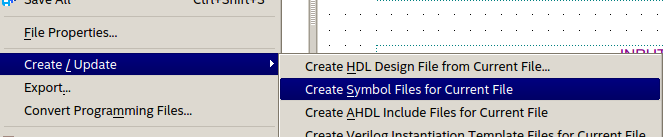
\includegraphics[scale=0.5]{images/MenuCreateSymbol.png}
\par}
\end{figure}

Simbol ini dapat kita gunakan untuk pada skematik lain dengan cara
yang sama ketika kita menambahkan gerbang logika dasar, yaitu dengan
mengklik icon \textbf{Symbol Tool}.

\begin{figure}[H]
{\centering
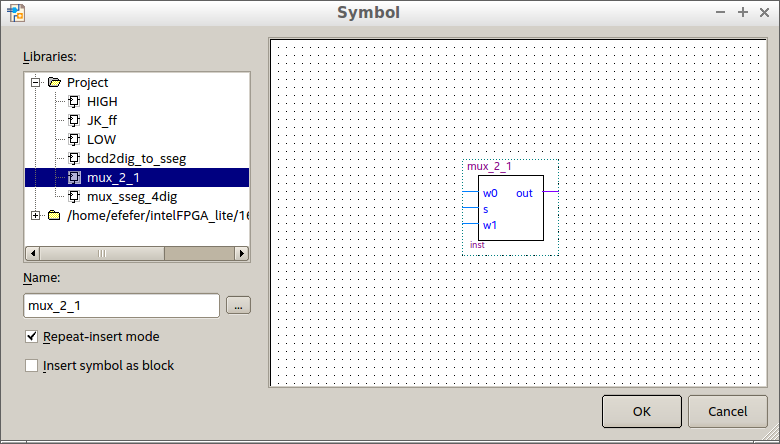
\includegraphics[scale=0.5]{images/symbol_mux_2_1.png}
\par}
\end{figure}

Contoh penggunaan (yang paling sederhana) dapat dilihat pada gambar berikut.

\begin{figure}[H]
{\centering
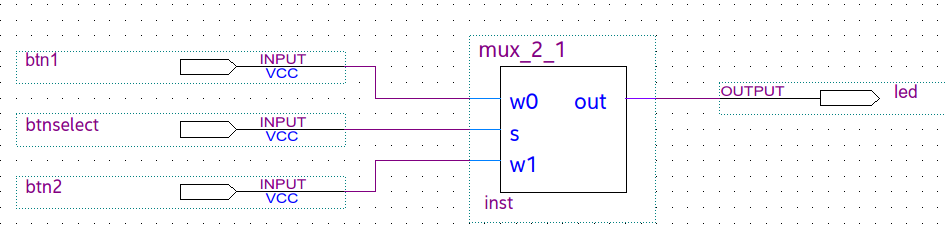
\includegraphics[scale=0.5]{images/tes_mux_2_1.png}
\par}
\end{figure}

